We will now discuss the Time Evolving Block Decimation (TEBD) algorithm for disoTPS, which can be used for both real and imaginary time evolution. The algorithm is a generalization of TEBD for MPS, which we discussed in Section \ref{sec:tensors_and_tensor_networks_matrix_product_states}. Analogously to MPS we start with a Suzuki-Trotter decomposition, approximating the time evolution operator $U\left(\Delta t\right) = e^{-i\Delta t \hat{H}}$ by a product of bond operators $U^{[x, y]}\left(\Delta t\right)$ acting only on neighbouring sites on the bond $[x, y]$. These bond operators then must be applied to the state in the correct order, while keeping the disoTPS structure intact. We will discuss the process of applying a single bond operator $U^{[x,y]}\left(\Delta t\right)$ to the disoTPS in Section \ref{sec:YB_isoTPS_TEBD_local_updates}. In Section \ref{sec:YB_isoTPS_TEBD_global_updates} we then discuss the full TEBD algorithm.

\subsection{Local TEBD updates}
\label{sec:YB_isoTPS_TEBD_local_updates}
\begin{figure}
	\centering
	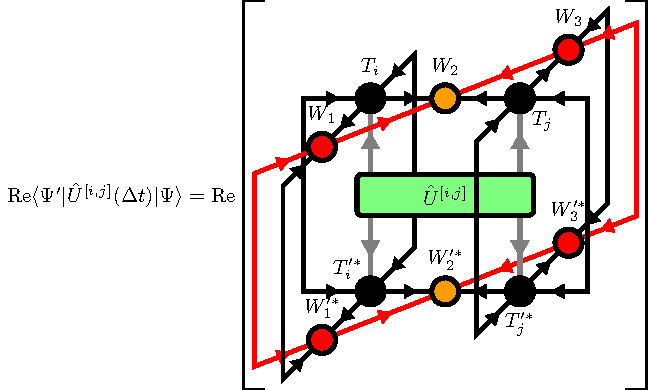
\includegraphics[scale=1]{figures/tikz/YB_isoTPS/tebd_environment/tebd_environment.pdf}
	\caption{The cost function of the optimization problem \eqref{eq:YB_isoTPS_TEBD_maximizing_overlap} that must be solved for locally applying TEBD operators $\hat{U}^{[i,j]} \coloneqq \hat{U}^{[i,j]}(\Delta t)$ can be computed as a contraction of the two-site wave functions of $\ket{\Psi}$ and $\ket{\Psi^\prime}$, sandwiching the operator between the two.}
	\label{fig:YB_isoTPS_TEBD_overlap_contraction}
\end{figure}
Let us assume that the orthogonality center is positioned between the two sites on which the bond operator $\hat{U}^{[x, y]}\left(\Delta t\right)$ acts. The five tensors around the orthogonality center then make up a sub-network with only incoming arrows, compare Figure \figref{fig:YB_isoTPS_twosite_expectation_value_environment}. We call these five tensors $T_1$, $T_2$, $W_1$, $W_2$ and $W_3$. The local TEBD update can then be formulated as the following problem: Find tensors $T_1^\prime$, $T_2^\prime$, $W_1^\prime$, $W_2^\prime$ and $W_3^\prime$ satisfying the isometry constraints and minimizing the error
\begin{equation}
	\label{eq:isoDTPS_TEBD_local_update_error}
	\varepsilon_\text{trunc} = \left\lVert \hat{U}^{[x,y]}(\Delta t)\ket{\Psi} - \ket{\Psi}\right\rVert
\end{equation}
Similar to the YB-move, we can rewrite this as the problem of maximizing the overlap
\begin{equation}
	\label{eq:YB_isoTPS_TEBD_maximizing_overlap}
	(T_{i,\text{opt}}^\prime, T_{j,\text{opt}}^\prime, W_{1,\text{opt}}^\prime, W_{2,\text{opt}}^\prime, W_{3,\text{opt}}^\prime)= \underset{T_i^\prime, T_j^\prime, W_1^\prime, W_2^\prime, W_3^\prime}{\argmax}\Re\bra{\Psi}\hat{U}^{[x,y]}(\Delta t)\ket{\Psi^\prime}.
\end{equation}
under the constraints $T_i^{\prime\dagger}T_i^\prime = \id$, $T_j^{\prime\dagger}T_j^\prime = \id$, $W_1^{\prime\dagger}W_1^\prime = \id$, $W_3^{\prime\dagger}T_3^\prime = \id$ and $\lVert W_2^\prime\rVert = 1$.
Using the isometry condition, the overlap $\bra{\Psi}\hat{U}^{[x,y]}(\Delta t)\ket{\Psi^\prime}$ can be computed by contracting the tensor network drawn in Figure \figref{fig:YB_isoTPS_TEBD_overlap_contraction}. For solving this problem we again use the Evenbly-Vidal algorithm. Similar to what we already did in Section \ref{sec:YB_move_iterative_local_optimization} for the YB move, we optimize one tensor at a time while keeping all other tensors fixed. This procedure is then repeated, sweeping over all five tensors until convergence is achieved. For more details on this optimization method see Appendix \ref{app:riemannian_optimization_of_isometries}. Since the time step $\Delta t$ is chosen to be small, the bond operator is close to identity, $\hat{U}^{[x,y]}(\Delta t)\approx\id$. Thus, a good initialization for the tensors of the updated wave function $\ket{\Psi^\prime}$ are simply the tensors of the old wave function $\ket{\Psi}$. \par
The computational complexity of applying a local bond operator to a disoTPS with the discussed algorithm scales as $\mathcal{O}(\chi^3D^3d^2) = \mathcal{O}(D^6)$. In practice it is observed that the algorithm converges after only a few iterations.

\subsection{Global TEBD updates}
\label{sec:YB_isoTPS_TEBD_global_updates}
\begin{figure}
	\centering
	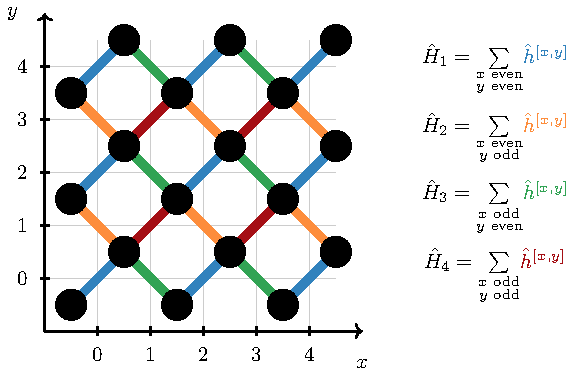
\includegraphics[scale=1]{figures/tikz/YB_isoTPS/tebd_global_update/tebd_global_update_a.pdf}
	\caption{A Hamiltonian $\hat{H}$ that is a sum of nearest-neighbour operators $h^{[x,y]}$ can be split into four parts made up of operators acting only on even/odd columns and even/odd bonds along a column.}
	\label{fig:YB_isoTPS_TEBD_global_update_TEBD1_splitting_and_TEBD2_chain}
\end{figure}
A global TEBD update evolves the state by a time $\Delta t$ and can be performed by applying local TEBD updates on all bonds. For each local TEBD update, the orthogonality center must be moved to the bond at which the update is applied. Because moving the orthogonality hypersurface can only be done approximately, the number of necessary moves should be minimized. \par
As we have already done for MPS in Section \ref{sec:tensors_and_tensor_networks_matrix_product_states}, let us assume that the Hamiltonian $\hat{H}$ can be written as a sum of nearest-neighbour operators. We index these nearest-neighbour operators $h^{[x, y]}$ by two integers $x$ and $y$ corresponding to the position of the orthogonality hypersurface and orthogonality center if moved to the bond on which $h^{[x,y]}$ acts. We define $x$ to increase from left to right and $y$ to increase from bottom to top, as shown in Figure \figref{fig:YB_isoTPS_TEBD_global_update_TEBD1_splitting_and_TEBD2_chain}. The Hamiltonian can then be split into four parts by first grouping the $h^{[x,y]}$ into two sets acting only on even and odd columns respectively and then splitting each set again into terms acting only on even/odd bonds along the respective columns. We can write this as
\begin{equation}
	\label{eq:YB_isoTPS_TEBD_splitting_local_Hamiltonian}
	\begin{split}
		\hat{H} = \sum_{x=1}^{2L_x-1} \sum_{y=1}^{2L_y-1}h^{[x,y]} &= \sum_{\substack{x\text{ even}\\y\text{ even}}} h^{[x, y]} + \sum_{\substack{x\text{ even}\\y\text{ odd}}} h^{[x, y]} + \sum_{\substack{x\text{ odd}\\y\text{ even}}} h^{[x, y]} + \sum_{\substack{x\text{ odd}\\y\text{ odd}}} h^{[x, y]} \\
		&\eqqcolon \hat{H}_1 + \hat{H}_2 + \hat{H}_3 + \hat{H}_4.
	\end{split}
\end{equation}
The operators appearing in the sum in $\hat{H}_j$ commute with each other and thus the exponential $e^{-i\Delta t\hat{H}_j}$ factorizes into a product of bond operators $\hat{U}^{[x, y]}(\Delta t) = e^{-i\Delta t\hat{h}^{[x, y]}}$. \par
We next use a Suzuki-Trotter decomposition to approximate the time evolution operator
\begin{equation}
	\label{eq:YB_isoTPS_TEBD_suzuki_trotter_first_order}
	\hat{U}(\Delta t) = \hat{U}^\text{TEBD1}(\Delta t) + \mathcal{O}(\Delta t^2)
\end{equation}
with
\begin{equation}
	\label{eq:YB_isoTPS_TEBD_first_order_TEBD_operator}
	\hat{U}^\text{TEBD}(\Delta t) \coloneqq e^{-i\Delta t\hat{H}_4} e^{-i\Delta t\hat{H}_3} e^{-i\Delta t\hat{H}_2} e^{-i\Delta t\hat{H}_1}.
\end{equation}
To evolve the state $\ket{\Psi}$ in time with this first order approximation we must compute $\ket{\Psi^\prime} \approx U^\text{TEBD1}(\Delta t)\ket{\Psi}$ as a disoTPS. The procedure is sketched in Figure \figref{fig:YB_isoTPS_TEBD_global_update_applying_TEBD1}. We start in the left-most column and apply all bond operators that act on bonds along this column. The bond operators on the column are applied in a brick-wall fashion analogously to the MPS algorithm: First all even bonds are updated and then all odd bonds are updated. Local updates are computed using the algorithm discussed in Section \ref{sec:YB_isoTPS_TEBD_local_updates}. Next, we move the orthogonality hypersurface two columns to the right and again apply all bond operators along the column. We proceed until all bond operators on even columns have been applied, in which case the orthogonality hypersurface is now positioned at its right-most position. We now sweep back to the left, applying all bond operators acting on odd columns along the way. Arriving back at the left-most column, all bonds making up $\hat{U}^\text{TEBD1}(\Delta t)$ have been applied in the correct order and the state has been evolved by time $\Delta t$. \par
\begin{figure}
	\centering
	\subcaptionbox{\label{fig:YB_isoTPS_TEBD_global_update_applying_TEBD1}}
	{%
		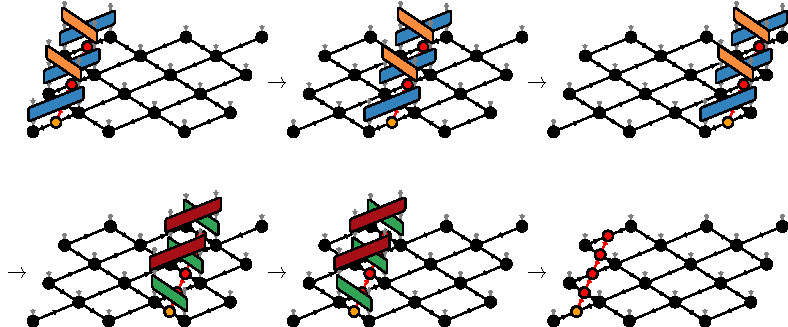
\includegraphics[scale=1]{figures/tikz/YB_isoTPS/tebd_global_update_steps/tebd_global_update_steps_a.pdf}
	}
	\par\bigskip\medskip
	\subcaptionbox{\label{fig:YB_isoTPS_TEBD_global_update_applying_TEBD2}}
	{%
		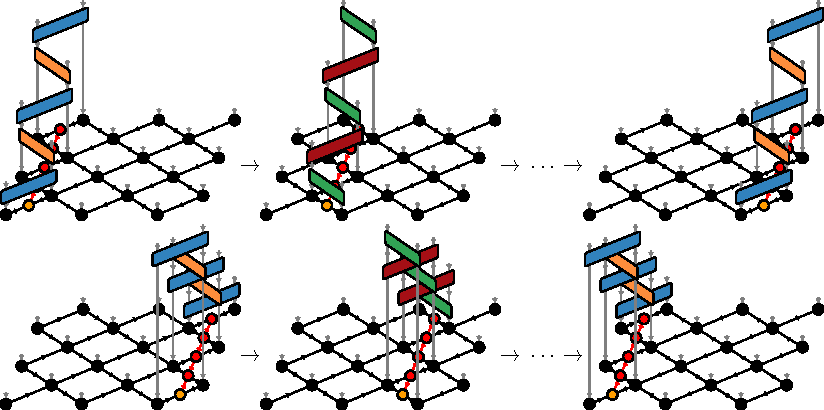
\includegraphics[scale=1]{figures/tikz/YB_isoTPS/tebd_global_update_steps/tebd_global_update_steps_b.pdf}
	}
	\caption{To apply a TEBD update, we sweep across the disoTPS once from left to right and back from right to left. (a) TEBD1 applies the operators in a brick-wall fashion, while (b) TEBD2 applies the operators along a chain.}
	\label{fig:YB_isoTPS_TEBD_global_update_applying_TEBD}
\end{figure}
We can obtain a better approximation of the time evolution operator $U(\Delta t)$ by performing a second order Suzuki-Trotter decomposition. By repeatedly applying the symmetrized decomposition
\begin{equation}
	e^{-i\varepsilon(A+B)} = e^{-i\frac{\varepsilon}{2}A}e^{-i\frac{\varepsilon}{2}A}e^{-i\varepsilon B} + \mathcal{O}(\Delta t^3)
\end{equation}
we obtain
\begin{equation}
	\begin{split}
		\label{eq:YB_isoTPS_tebd_second_order_suzuki_trotter_decomposition}
		e^{-i\Delta t\hat{H}} &= \exp\left(-i\Delta t\sum_{x,y}\hat{h}^{[x,y]}\right) \\
		&= e^{-i\frac{\Delta t}{2}\hat{h}^{[1, 1]}} e^{-i\Delta t\left(\hat{H}-\hat{h}^{[1,1]}\right)} e^{-i\frac{\Delta t}{2}\hat{h}^{[1, 1]}} + \mathcal{O}(\Delta t^3)\\
		&= e^{-i\frac{\Delta t}{2}\hat{h}^{[1, 1]}} e^{-i\frac{\Delta t}{2}\hat{h}^{[1, 2]}} e^{-i\Delta t\left(\hat{H}-\hat{h}^{[1,1]}-\hat{h}^{[1, 2]}\right)} e^{-i\frac{\Delta t}{2}\hat{h}^{[1, 2]}} e^{-i\frac{\Delta t}{2}\hat{h}^{[1, 1]}} + \mathcal{O}(\Delta t^3)\\
		&=\cdots\\
		&= e^{-i\frac{\Delta t}{2}\hat{h}^{[1, 1]}} e^{-i\frac{\Delta t}{2}\hat{h}^{[1, 2]}} \cdots e^{-i\frac{\Delta t}{2}\hat{h}^{[1, 2]}} e^{-i\frac{\Delta t}{2}\hat{h}^{[1, 1]}} + \mathcal{O}(\Delta t^3).
	\end{split}
\end{equation}
Here, in each step we "split off" one operator $\hat{h}^{[x,y]}$ from the sum. The final result is a product of bond operators $\hat{U}^{[x,y]}(\Delta t/2))$ that must be applied from right to left. The algorithm of applying a global second order update is thus similar to a TEBD update of first order. We sweep across the disoTPS once from left to right and back, applying bond operators along the way in the correct order, as visualized in Figure \figref{fig:YB_isoTPS_TEBD_global_update_applying_TEBD2}. The difference to TEBD1 is that now the operators are applied in a chain-like order instead of the brick wall order of TEBD1. The number of YB moves for TEBD1 and TEBD2 is the same, but the smaller Trotter error of $\mathcal{O}(\Delta t^3)$ instead of $\mathcal{O}(\Delta t^2)$ allows us to use larger time steps for TEBD2, resulting in a smaller number of YB moves per unit time. We find that the YB move is the primary source of error in practice and thus expect TEBD2 to perform much better than TEBD1. \par 
In principle, one could also go to higher decomposition orders \cite{cite:finding_exponential_product_formulas_of_higher_orders}. However, already a third order decomposition would necessitate a larger number of sweeps for applying the full update, increasing the error accumulated through YB moves. It is therefore not clear if higher order decompositions would be able to improve the method further.
